%%%%%%%%%%%%%%%%%%%%%%%%%%
% MSc Project Background Report Template
% Prof. Roger K. Moore
% University of Sheffield
% 22 March 2017
%%%%%%%%%%%%%%%%%%%%%%%%%%


\documentclass[11pt,oneside]{book}
\usepackage[margin=1.2in]{geometry}
\usepackage{setspace}
\usepackage[toc,page]{appendix}
\usepackage[none]{hyphenat} % turn hyphenation off by default
\usepackage{graphicx}
\usepackage{pgfgantt}

\begin{document}

\frontmatter

\begin{titlepage}

% You need to edit the details here

\begin{center}
{\LARGE University of Sheffield}\\[1.5cm]
\linespread{1.2}\huge {\bfseries Building a Speaker Diarization System for the DIHARD II Challenge}\\[1.5cm]
\linespread{1}

\includegraphics[width=5cm]{images/tuoslogo.png}\\[1cm]
{\Large Mangesh Hemant Hambarde}\\[1cm]
{\large \emph{Supervisor:} Dr. Thomas Hain}\\[1cm]
\large A report submitted in fulfilment of the requirements\\ for the degree of MSc Computer Science with Speech and Language Processing\\[0.3cm] 
\textit{in the}\\[0.3cm]
Department of Computer Science\\[2cm]
\today
\end{center}

\end{titlepage}

% -------------------------------------------------------------------
% Declaration
% -------------------------------------------------------------------

\newpage
\chapter*{\Large Declaration}

\setstretch{1.1} % set the line spacing differently if you wish, but this looks good to me. 

All sentences or passages quoted in this report from other people's work have been specifically acknowledged by clear cross-referencing to author, work and page(s). Any illustrations that are not the work of the author of this report have been used with the explicit permission of the originator and are specifically acknowledged. I understand that failure to do this amounts to plagiarism and will be considered grounds for failure in this project and the degree examination as a whole.\\[1cm]

\noindent Name:\\[1mm]
\rule[1em]{25em}{0.5pt}

\noindent Signature:\\[1mm]
\rule[1em]{25em}{0.5pt}

\noindent Date:\\[1mm]
\rule[1em]{25em}{0.5pt}

% -------------------------------------------------------------------
% Abstract
% -------------------------------------------------------------------

\chapter*{\Large \center Abstract}

Speaker Diarization is commonly known as the task of finding out ``who spoken when?" in an audio recording. It is an important field because it is a crucial preprocessing step for many other areas in speech technology. One of the key challenges faced in this field is how to deal with domain variation. There is a lot of speaker, channel and environment variability that exists in the speech signal. Most previous diarization research has focused on specific domains and performance on diverse datasets is expected to be poor. DIHARD is a challenge that has been created by the diarization research community to boost research in the area of diverse datasets. The main aim of the project is to build a complete speaker diarization system that works within the rules of the 2019 DIHARD challenge using the Kaldi toolkit. The system is not officially submitted to the challenge because the dissertation timeline did not allow it. Several different system configurations are explored in the project. The best system involved concatenating two different speaker embeddings into a single embedding. This resulted in a diarization error rate (DER) of 24.64\% on the evaluation set, almost a 7.3\% relative improvement compared to the baseline which was at 26.58\%.



% -------------------------------------------------------------------
% TOC etc
% -------------------------------------------------------------------

\tableofcontents
\listoffigures
\listoftables

\setstretch{1.1} 

\mainmatter

\chapter{Introduction}

Speaker diarization is the task of finding out ``who spoke when?" in an audio recording with an unknown amount of speakers. It aims to find all segments of speech within the recording, possibly overlapping, along with their intra-recording speaker identities. It acts as an important upstream preprocessing step for most tasks in speech processing, like speech recognition, speech enhancement, speech coding etc.

With increase in computing power, speech processing technologies have achieved incredible advances in the past decade that were not possible earlier. This has increased interest in Rich Transcription (RT) technologies that can be used to automatically index the enormous amount of audio and video information that is generated in the modern world. Since speaker diarization is an important part in any RT system, there is a great deal of research interest in the area.

Diarization is not an easy problem since the output is affected by several factors like the application domain (broadcast news, meetings, telephone audio, internet audio, restaurant speech, clinical recordings etc), types and quality of microphones used (boom, lapel, far-field), inter-channel synchronization problems, overlapping speech, etc. These days, most of the research focuses on the meeting speech domain, since most problems that exist in speech recognition are encountered in this domain. The meeting scenario is thus often termed as ``speech recognition complete".

The DIHARD challenge was created to establish standard datasets for diarization and create performance baselines for comparison, thus encouraging further research. The challenge focuses on ``hard" diarization, combining several domains of speech like broadcast speech, meeting speech, telephone speech, and many more. Creating a system for the challenge can be a rewarding experience since it gives a chance to learn about state-of-the-art speaker diarization techniques.

\section{Speaker Diarization}

\section{Motivation and Objectives}

\section{Report Outline}


\chapter{Literature Survey}

\section{Introduction}

\begin{figure}[h]
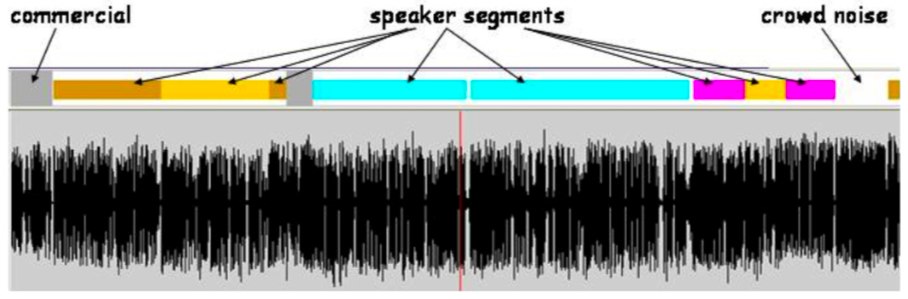
\includegraphics[width=12cm]{figures/diarization.png}
\centering
\caption{Example of audio diarization on broadcast news \cite{1677976}}
\label{fig:diarization}
\end{figure}

\section{Diarization System Modules}

Given below in figure \ref{fig:modules} is the general organization of the modules of a diarization system. Later, a brief overview of each diarization system module is given.

\begin{figure}[ht]
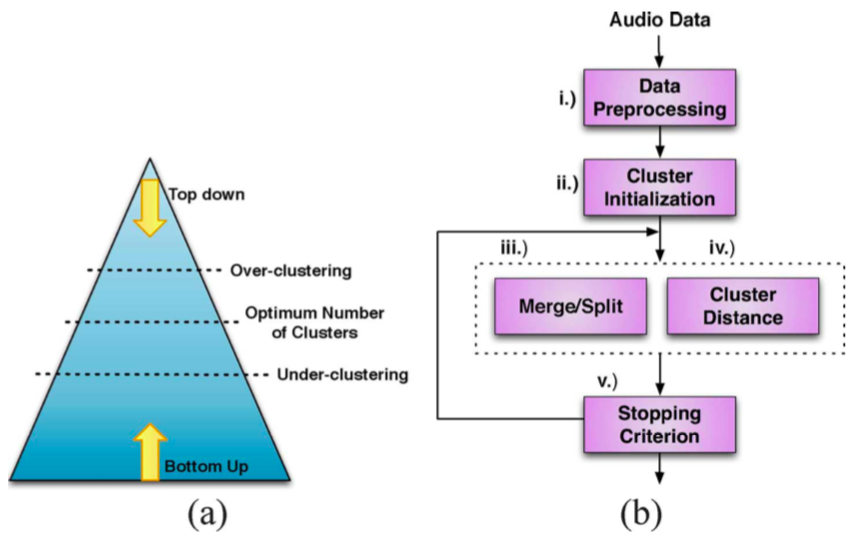
\includegraphics[width=15cm]{figures/modules.png}
\centering
\caption{General Diarization system. (a) Alternative clustering schemas. (b) General speaker diarization architecture. \cite{anguera2012speaker} }
\label{fig:modules}
\end{figure}

	\subsection{Preprocessing}
		\subsubsection{Speech Enhancement / Noise Reduction}
		A diarization system needs to address the problem of environmental noise in audio recordings. It is important to remove as much background noise as possible, but also speaker-specific information should not be lost. Also, the artefacts in denoised speech tend to reduce diarization performance. In recent years deep learning methods have partially solved the problem of artefacts, as shown in \cite{6739096}, \cite{6639038}, \cite{6665000}. But generalization ability in mismatched conditions (in terms of speaking style, interferences, interaction) is still a problem. After this stage, the enhanced speech results in increased performance for the subsequent diarization stages. 
		
		\subsubsection{Multiple Microphones}
		In the meeting domain, multiple microphones are often used from different locations of the room, so there are multiple channels of audio available to work with. Multiple microphones allow the possibility of choosing the channel with the best signal-to-noise ratio (SNR) but that also means dealing with inter-microphone delays. Many approaches have been designed to do diarization with multiple microphones. One approach performs diarization on each channel separately and merge the outputs using some algorithm. Another approach does speaker segmentation on all channels separately but only applies diarization on segments with best SNR. Some systems also combine channels to obtain a single mono channel, possibly weighing them by their SNR, then performing the diarization on it.
		
		\subsubsection{Acoustic Beamforming}
		Multiple channels usually come with inter-channel delay (which can be in the order of seconds) with arises due to the time-delay-of-arrival (TDOA) of each microphone. This is a huge problem and severely affects diarization performance. This is commonly solved by acoustic beamforming which is discussed in \cite{anguera2007acoustic}. Many people use the free tool BeamformIt \cite{anguera2006beamformit} which uses an enhanced delay-and-sum algorithm to correct misalignments.

	\subsection{Speech Activity Detection}
	Speech activity detection splits a recording into speech and nonspeech segments. This is important because this obviously has a large effect on the diarization output. The task is far from trivial since nonspeech can consist of a variety of sounds; for example in a meeting setting, it can consist of paper shuffling, door knocks, breathing, coughing, laughing etc.
	The general approach to doing speech activity detection is model-based. The binary classification models are pre-trained with external speech and non-speech data. This also makes it possible to adapt them to specific domains. This process does have a drawback because relying on external data makes the models less robust to changes in acoustic conditions. Hybrid approaches are one proposed solution, in which an energy detector is first used to label a limited amount of data for which there is high confidence in the classification. In the next step, this labelled data is used to train models that are specific to the recording event. These models are later used to obtain the final segmentation.
	
	\subsection{Segmentation}
	Another fundamental part of speaker diarization systems is speaker segmentation. The goal of this stage is to split the audio stream into speaker homogeneous segments, or in other words, detecting speaker turns. The classical approach to segmentation uses a sliding window across the speech segments, comparing consecutive windows. The comparison decides whether the two segments are better accounted by two separate models (different speakers) or a single model (same speaker) using a empirically determined threshold. Many distance metrics exist for making this decision, some of which include the $\Delta$ Bayesian Information Criterion ($\Delta$BIC) metric \cite{Chen1998SpeakerE}, generalized likelihood ratio (GLR), Kullback-Leibler (KL) divergence etc, information change rate (ICR) etc.
		
	\subsection{Clustering}

\begin{figure}[h]
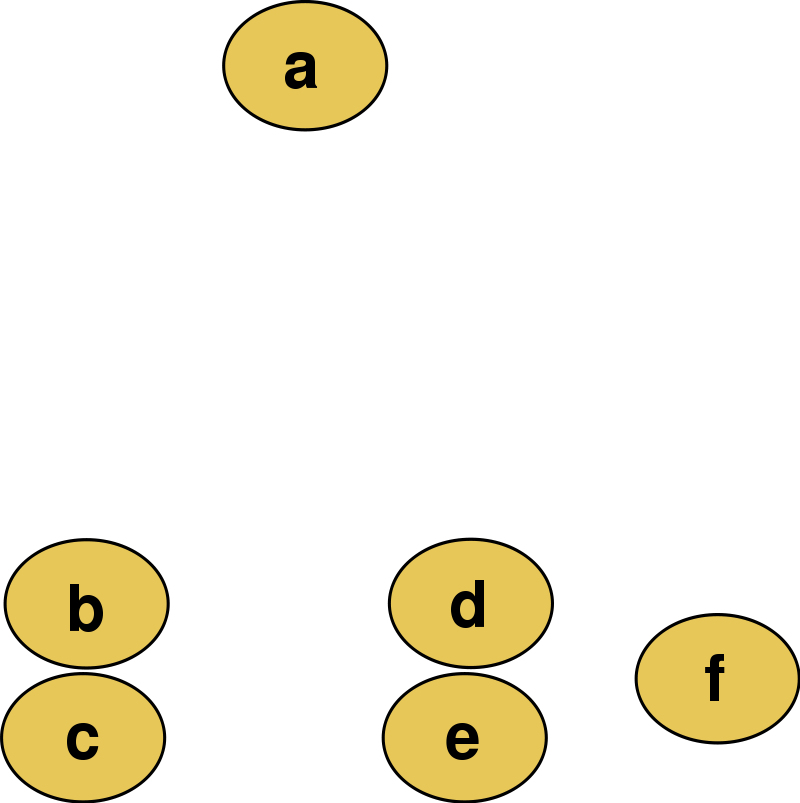
\includegraphics[width=4cm]{figures/hac-1.png}
\centering
\caption{Unclustered data \cite{wiki:hac}}
\label{fig:hac1}
\end{figure}	
	
	The segmentation step works on adjacent windows, but clustering works on the whole audio stream and works to group together all same-speaker segments. In the ideal case, every speaker has their own cluster. The same distance metrics as previous can be used here too. Most diarization systems fall in two categories: bottom-up and top-down clustering approaches. Regardless of the approach used, both of them try to converge to the optimum number of speakers, which is the actual number in the audio recording. If the final number is high than the actual number, the system is said to be under-clustered. If lower then it is called over-clustered. Both approaches are based on Hidden Markov Models (HMMs) where each state is a Gaussian Mixture Model (GMM) and represents a speaker. State transitions correspond to speaker turns. Each cluster is modelled with a GMM.
	
\begin{figure}[h]
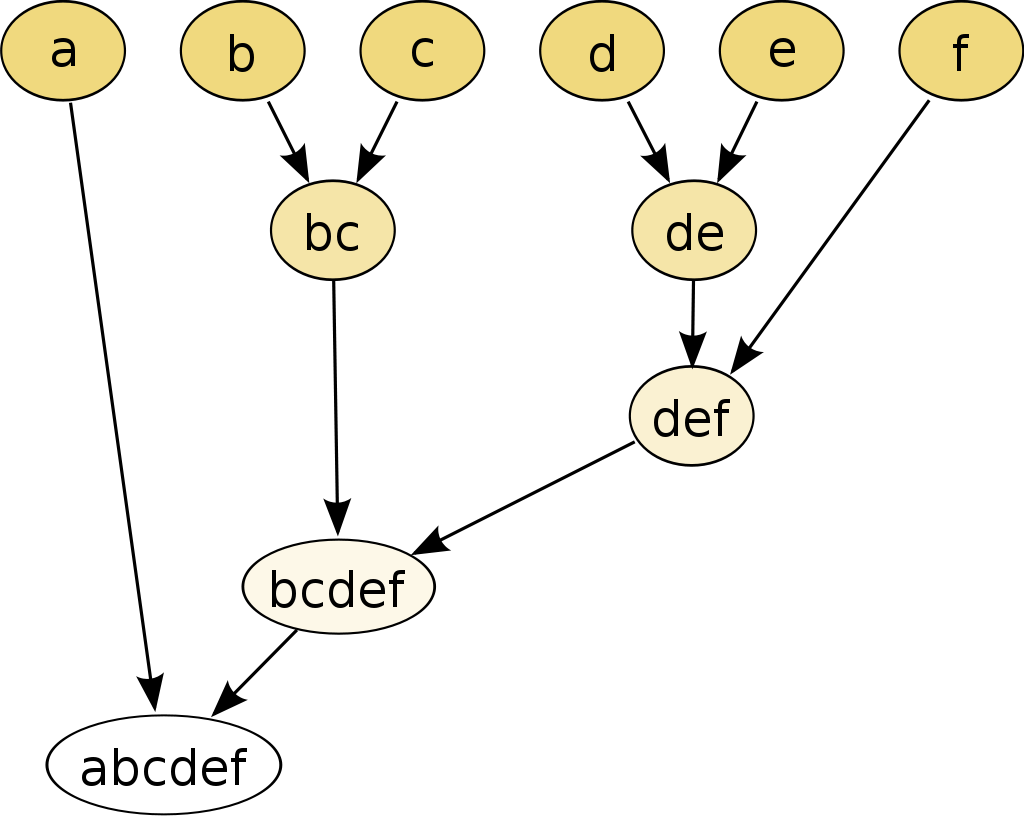
\includegraphics[width=6cm]{figures/hac-2.png}
\centering
\caption{AHC \cite{wiki:hac}}
\label{fig:hac2}
\end{figure}
	
	The bottom-up approach is the most commonly used one. It is also known as agglomerative hierarchical clustering (AHC). This approach initializes many more clusters than the actual speakers and aims at reducing the number of clusters by 1 in each iteration by merging two of the clusters. Many initializations are possible, some use k-means clustering and many use uniform initialization. Merged clusters are modelled with a GMM and use the data from the two individual clusters. Reassignment of frames to clusters is done after each cluster merge using Viterbi decoding. The whole process is repeated until some stopping criterion is reached.
		
	The top-down approach is far less popular and uses just one model (GMM) as a starting point which models the whole audio and successively adds models. Initially all segments are marked unlabelled.  Some unlabelled segments are chosen using some selection process, and used as training data for a new model (GMM). These segments are marked labelled. Viterbi alignment is interleaved and the models are re-adapted. This is continued until some stopping criterion is reached (similar to the bottom up case) or no unlabelled segments remain. Top down systems are usually out-performed by bottom up systems, but they have an advantage of being computationally efficient.
	
	Alternately, Bayesian machine learning has also been used for diarization. The key here is not making point estimates of system parameters, but instead the parameters of their distribution, also known as hyperparameters. This allows soft decisions to be taken and thus avoids a premature hard decision. However this needs computation of posterior distributions which are often too complex, and thus approximate inference methods are needed. Monte Carlo Markov Chains (MCMCs) made using Bayesian possible by computing distributions via sampling, but they are often too slow with large amount of data. An  alternative approach was Variational Bayes \cite{10.1007/11677482_27} \cite{Reynolds2009ASO} \cite{Kenny2008BayesianAO} is popular for approximating distributions, which allows approximating the intractable distribution by converting the inference problem to an optimization problem.
	
	\subsection{One-step segmentation and clustering}
	In an approach where clustering is a separate step which is performed after segmentation, there is no provision for splitting segments which contain a speaker turn, thus the quality of diarization is good only if the initial segmentation is of good quality. Since this is rarely the case, one-step segmentation and clustering approaches have been introduced which combine clustering with iterative re-segmentation. These systems perform clustering on a frame-to-cluster basis. Viterbi realignment is used to re-segment the audio based on the current clustering hypothesis, and the models are retrained based on the new segmentation. Most of the state-of-the-art diarization systems use one-step segmentation and clustering.
	
	\subsection{Speaker Representation}
		\subsubsection{GMM-UBM model}
		Early diarization systems used GMMs with cepstral features to represent speakers. However, since segments durations are small, the number of feature vectors available is often too small to estimate a GMM. To solve this, a pre-trained Universal Background Model (UBM) was introduced \cite{Reynolds:2000:SVU:2774258.2774423}, which is trained from a large number of speakers from an external dataset to capture the general variability of speech. To get the speaker model, the UBM is adapted to the speaker segments. To compute statistical similarity between GMMs, measures like KL divergence, normalized cross likelihood ratio (NCLR) can be used.
				
		\subsubsection{GMM supervectors}
		Experiments show that the means of GMMs have the most amount of speaker information by far. So the mean vectors of a GMM are concatenated into a giant vector called a GMM supervector, and it represents the GMM. Distance measures between supervectors have been investigated in \cite{5545402}. Two supervectors can only be compared if they are adapted from the same UBM.
		
		\subsubsection{i-vectors}
		The high dimensionality of supervectors is a problem for computation. \cite{5545402} uses factor analysis to reduce the dimensionality of the supervector and get a new representation into a new space called ``total variability subspace". The representation obtained is called i-vector. The parameters to do this transformation need to be learned from a training dataset. Recently i-vectors have been shown to give state-of-the-art results in speaker recognition.
				
	\subsection{Overlapping Speech}
	Most speaker diarization systems assign only one speaker to each segment. This can be considered as a fundamental limitation, since it is entirely possible for a segment to have overlapping speech from multiple speakers. In such segments, both missed speech errors and speaker identification errors occur. These segments also affect the purity of clusters of which they are a part of.
	Some strategies have been used to deal with segments of overlapping speech. In systems where ground-truth overlap detection was available, some have tried to add a second speaker to these regions by just using speaker labels of neighbouring segments. Some have also tried excluding overlapping regions from the input to the diarization system. Real overlap detection has been done in the past \cite{trueba2008handling} using a 3-state HMM-GMM system (nonspeech, non-overlapped speech, overlapped speech) with some success. Very recently, \cite{isik2016single} and \cite{hershey2016deep} talk about doing speaker separation for single-channel mixtures using a deep learning architecture called ``deep clustering".
	
	\subsection{Time-Delay Features}
	As already seen, inter-channel delays exist in multi-channel scenarios. It is possible to use these delays for speaker localization. These estimates of speaker location (assuming that speakers do not move) can be treated as alternative features.
	
	\subsection{Diarization Evaluation}
	Since 2004, the National Institute of Standards and Technology (NIST) organizes benchmark evaluations within the RT campaigns. One of the tasks is speaker diarization. Most of recent NIST RT evaluations have focussed on the conference meeting domain which is more challenging and as stated before, ``speech recognition complete". Several evaluation conditions are created using combinations of different conditions - single/multi channel audio, microphone types etc.
	
	\subsubsection{Diarization Error Rate}
		The NIST systems are evaluated using the diarization error rate (DER) metric, which is composed of three errors: missed speech (MISS), false alarm speech (FA), and speaker error (ERROR). TOTAL is the total duration of the audio recording. Missed speech is the percentage of speech that is in the ground truth but not in the prediction. False alarm speech is the percentage of speech that is in the prediction but not in the ground truth. Speaker error is the percentage of speech assigned to an incorrect speaker. Speaker error is classified into incorrectly assigned single speaker, and speaker overlap error. Speaker overlap error can be further classified as missed overlap (few speakers predicted than actual) or false alarm overlap (more speakers predicted than actual).
		From the definition of DER it is obvious that it is time-weighted. It assigns more importance to the diarization quality of speakers who have longer speaking times. Sometimes a non-scoring collar of a few milliseconds is applied on the sides of ground-truth segment boundaries to account for inconsistencies caused by imprecise start and end timestamps.
			
	$$ DER = \frac{FA + MISS + ERROR}{TOTAL} $$

	\subsubsection{Jaccard Error Rate}
	A new metric has been developed for DIHARD for use as an alternative metric called the Jaccard Error Rate (JER). This is based on the Jaccard Index \cite{hamers1989similarity}. The Jaccard Index is computed for each pair of optimal mappings between reference and system speakers. The Jaccard Error Rate is defined as 1 minus the average of these scores. It is similar to DER, but unlike DER it weighs each speaker's contribution equally regardless of how much they speak.
	
	Assume we have $N$ reference speakers, $M$ system speakers. After the optimal mappings are determined, for each reference speaker $ref$ the speaker-specific Jaccard error rate $JER_{ref}$ is computed by:
	
	$$ JER_{ref} = \frac{FA + MISS}{TOTAL} $$
	
	The Jaccard error rate is then the average of speaker specific Jaccard error rates.
	
	$$ JER = \frac{1}{N} \sum_{ref} JER_{ref} $$

\section{Summary}
	To summarize, we can see that even a seemingly simple problem statement like speaker diarization has a lot of modules doing various jobs under the hood. The core of the system is the segmentation and clustering part, which does most of the work. Diarization uses a lot of concepts from the fields of speaker identification and verification for modelling speakers.

\chapter{Baseline setup}

\section{Overview}
There are three software baselines provided by the DIHARD II organizers, each for the parts of speech enhancement, speech activity detection and diarization. The speech enhancement baseline and the speech activity detection are meant to be used together in the case of system-generated SAD (tracks 2 and 4), but since we only work with reference SAD, we do not need them. Thus we will only describe the diarization baseline in the following sections.

The diarization baseline is based on the best performing submission \cite{sell2018diarization} from John Hopkins University (JHU) in the previous year's DIHARD challenge (DIHARD I). There are 4 Kaldi recipes, each for an evaluation track, but we will focus only on the recipe for Track 1 since we only work with single channel audio and gold speech segmentation.

\section{DIHARD datasets}


\section{Baseline directory structure}
The baseline repository is localted at \ttvar{https://github.com/iiscleap/DIHARD_2019_baseline_alltracks} and has the following directory structure. Some of the irrrelevant files have been removed.

\begin{verbatim}
DIHARD_2019_baseline_alltracks/
|-- data
|   |-- final.raw
|   |-- max_chunk_size
|   |-- min_chunk_size
|   |-- plda_track1
|   |-- plda_track2
|   |-- plda_track3
|   |-- plda_track4
|-- README.md
|-- recipes
|   |-- track1
|   |-- track2
|   |-- track2_den
|   |-- track3
|   |-- track4
|   `-- track4_den
|-- scripts
|   |-- alltracksrun.sh
|   |-- flac_to_wav.sh
|   |-- make_data_dir.py
|   |-- md_eval.pl
|   |-- prepare_feats.sh
|   |-- prep_eg_dir.sh
|   `-- split_rttm.py
`-- tools
    |-- env.sh
    |-- install_dscore.sh
    |-- install_kaldi.sh
}
\end{verbatim}

The \ttvar{data} directory has pre-trained models (in Kaldi binary format) and some configuration parameters - \ttvar{final.raw} is the neural network x-vector extractor, and the \ttvar{plda_*} files are the PLDA backends for the 4 tracks. The \ttvar{recipes} directory has the \ttvar{run.sh} files for all 4 recipes, we only care about \ttvar{track1}. The scripts directory has extra scripts that are needed on top of the \ttvar{egs/dihard_2018} Kaldi recipe - \ttvar{alltracksrun.sh} is the main diarization script, \ttvar{make_data_dir.py} makes the Kaldi data directory from the DIHARD datasets (creating files like wav.scp, segments, utt2spk etc), \ttvar{prep_eg_dir.sh} copies the extra files from this repository to the \ttvar{egs/dihard_2018} directory, \ttvar{md_eval.pl} \cite{mdeval2006} is a diarization evaluation script that was developed by NIST, and others are self-explanatory. The \ttvar{tools} directory holds scripts to install Kaldi and dscore \cite{dscore}, which are installed in the same directory.

The baseline code modifies and reuses the \ttvar{egs/dihard_2018} recipe that was checked into Kaldi by the researchers at JHU. It does this by copying over new scripts and data that is needed to the \ttvar{egs/dihard_2018} directory, \ttvar{cd}'ing to that directory and running the recipe from there.

We modify and add scripts in this repository so we can easily run experiments with different parameters. The \ttvar{run.sh} script is modified to allow easily changing parameters to run different experiments.

\section{Initial segmentation}
The initial segmentation step is done by \ttvar{make_data_dir.py}. It deals with separating speech and non-speech segments from the recording files using the reference SAD which is provided in the form of HTK label files (.lab). Each audio recording has one label file. The label file has one line for each speech segment with the format \ttvar{<start-timestamp> <end-timestamp> speech}.

\begin{verbatim}
0.000 3.513 speech
4.698 7.133 speech
7.377 12.826 speech
13.284 16.797 speech
17.312 21.201 speech
...
\end{verbatim}

This results in a bunch of segments which are known to be containing only speech. These are treated as ``utterances" in Kaldi terminology and act as keys in the \ttvar{utt2spk}, \ttvar{feats.scp} and \ttvar{segments} files. These files reside in two Kaldi ``data directories", one for each dev and eval.

\section{Features}
The baseline then extracts 30 dimensional MFCC features for each of the every 10 ms using a 25 ms window. It uses the standard \ttvar{steps/make_mfcc.sh} Kaldi script for this. The MFCC configuration used \ttvar{mfcc.conf} is given below.

\begin{verbatim}
--sample-frequency=16000
--frame-length=25 # the default is 25
--low-freq=20 # the default.
--high-freq=7600 # Nyquist (8k in this case).
--num-mel-bins=30
--num-ceps=30
--snip-edges=false
\end{verbatim}

Later, cepstral mean and variance normalization (CMVN) with a 3 second sliding window is applied using the \ttvar{apply-cmvn-sliding} Kaldi tool.

\section{Subsegmentation}
After MFCC features are ready, the utterances are uniformly divided into smaller 1.5 second subsegments with a 0.75 second overlap. This creates new Kaldi data directories (one each for dev and eval sets) with newer keys corresponding to each subsegment. An x-vector is extracted from each of these subsegments in the next step using the Kaldi binary \ttvar{nnet3-xvector-compute}.

\section{Speaker representation}
The baseline extracts an 512-dimensional x-vector from each subsegment using a neural network x-vector extractor. The extractor is trained on the datasets VoxCeleb I and II, along with added augmentation. Utterances smaller than 400 frames and speakers less than 8 utterances are discarded. Since the VoxCeleb dataset does not come with gold speech segmentation, the program \ttvar{compute-vad} is used with the following configuration to classify each frame into speech or non-speech.

\begin{verbatim}
--vad-energy-threshold=5.5
--vad-energy-mean-scale=0.5
--vad-proportion-threshold=0.12
--vad-frames-context=2
\end{verbatim}

It uses simple energy-based thresholding to generate a speech segmentation. Finally there are 1,277,503 utterances spoken by 7,351 speakers that can be used for training. Although the actual number is much more because of augmentation.

The augmentation is done by additive noise (noise, music, babble) using the MUSAN dataset and reverberation using the RIR dataset. The augmentation is done because it was determined in \cite{snyder2018x} that x-vectors exploit large quantities of training data much better than i-vectors, and show a significant increase in performance.

\section{Scoring}
For scoring two x-vectors, a PLDA backend is used as a distance metric. To train the PLDA backend, x-vectors are extracted from a random subset (size 128k) of the VoxCeleb dataset. To adapt the extracted x-vectors to the DIHARD domain, they are whitened with a whitening transform learned from the DIHARD development set. The PLDA model is trained using the x-vectors and the \ttvar{ivector-compute-plda} Kaldi binary.

Each pair of x-vectors within a recording is then scored using the PLDA backend by reusing \ttvar{score_plda.sh} from \ttvar{egs/callhome_diarization}. These scores are stored as an affinity matrix for each recording.

\section{Clustering}
The x-vectors are then clustered using agglomerative hierarchical clustering (AHC) and a parameter sweep is done on the dev set to find the threshold that maximises the DER on the dev set. This threshold is then used for clustering the x-vectors of the eval set. The \ttvar{agglomerative-cluster} Kaldi binary is used for clustering.

\section{Diarization output}
The clustering output is used to generate RTTMs using the script \ttvar{make_rttm.py} from \ttvar{egs/callhome_diarization}. The RTTMs give a flat segmentation of the recordings with no overlap. Since the x-vectors were extracted from segments that were overlapping, care needs to be taken when two adjacent segments are assigned to a different speaker. The script places the speaker boundary midway between the end of the first segment and the start of the second segment.


\chapter{Experiments and Results}

	\section{Baseline results}
	
	\section{Using Existing Pre-trained Models}
		\subsection{Kaldi VoxCeleb x-vector model}
		\subsection{Kaldi VoxCeleb i-vector model}
	
	\section{Training Models on In-Domain Data}
		\subsection{No Augmentation}
		\subsection{Augmentation with Noise and Reverberation}
		
	\section{Manual Speech Activity Detection}
		\subsection{WebRTC}
		\subsection{SHoUT toolkit}
		\subsection{Energy-based}
		\subsection{DNN-based}
		
	\section{Speech Enhancement}
		\subsection{Baseline}
	
	\section{Alternative Distance Metrics for Clustering}
		\subsection{BIC}
		\subsection{Cosine}
		
	\section{Feature concatenation}
		\subsection{Concatenating i-vectors and x-vectors}
	
	\section{Tuning Hyperparameters}
		\subsection{Vector Dimensionality}
		\subsection{Segment Length and Overlap}
		\subsection{Clustering Threshold}
		\subsection{Number of UBM Gaussians}
	
	\section{Cluster Purity Scores}
	
	\section{Breaking down DER}
		\subsection{By amount of speaker data}
		\subsection{By recording}
		\subsection{By utterance duration}
		\subsection{By number of speakers}
\chapter{Conclusions}



\bibliographystyle{acm}
\bibliography{main}

\end{document}
